\documentclass[12pt,a4paper]{article}

\usepackage[utf8]{inputenc}
\usepackage[T2A]{fontenc}
\usepackage[ukrainian]{babel}

\usepackage{geometry}
\geometry{left=2cm,right=2cm,top=2cm,bottom=2cm}
\usepackage[table]{xcolor}
\usepackage{graphicx}
\usepackage{placeins}
\usepackage{array,multirow}
\usepackage{booktabs}
\usepackage{caption}
\renewcommand{\thetable}{№\arabic{table}}
\captionsetup[table]{name=Таблиця}

\usepackage{amsmath}
\usepackage{pdflscape}
\usepackage{hyperref}

\begin{document}

    \begin{titlepage}

        % Картинка шапки (по центру, з відступом від верху)
        \begin{center}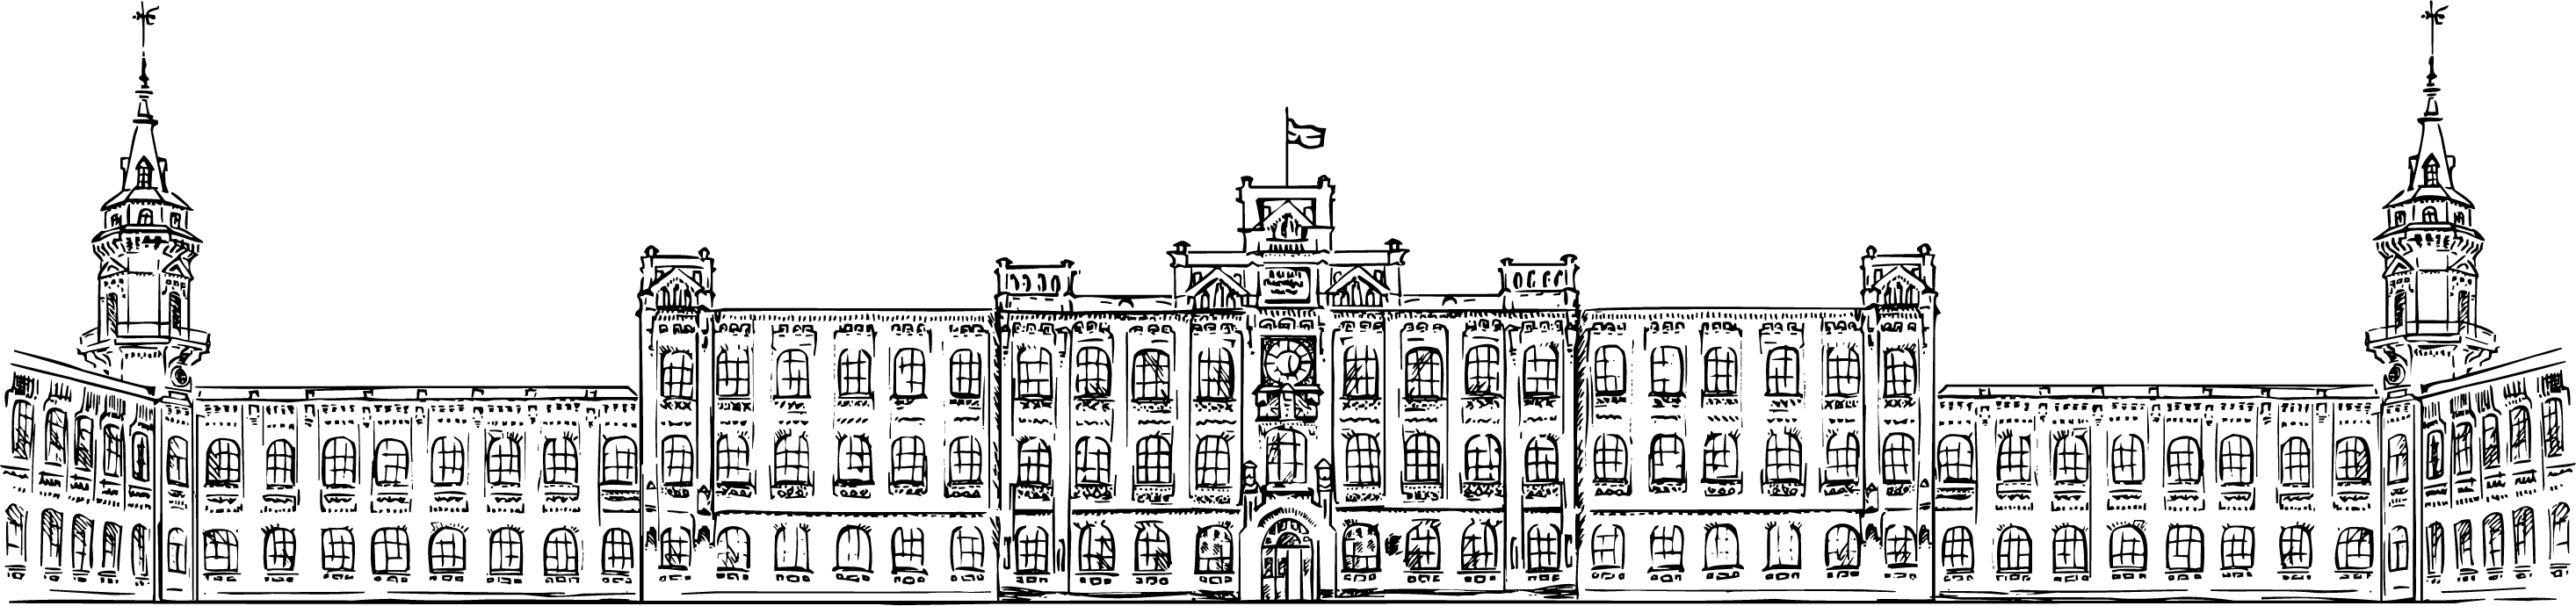
\includegraphics[width=0.7\textwidth]{../../../TITLES/letterhead.png}\end{center}

        \begin{center}
            \large Національний технічний університет України\\
            «Київський політехнічний інститут імені Ігоря Сікорського»\\[1em]
            Факультет інформатики та обчислювальної техніки\\
            Кафедра обчислювальної техніки
        \end{center}

        \vfill

        \begin{center}
            \textbf{\LARGE Практична електроніка}\\[2em]
            \textbf{\Large Лабораторна робота №7}\\[0.5em]
            «Дослідження аналого-цифрових перетворювачів (АЦП)»
        \end{center}

        \vfill

        \begin{flushright}
            Виконав: студент 2 курсу ФІОТ, гр. ІО-41\\
            \textit{Давидчук А.~М.}\\[1em]
            Перевірив: \textit{Гайдай А.~Р.}
        \end{flushright}

        \vfill

        \begin{center}Київ --- 2025\end{center}

    \end{titlepage}

    % Основний документ:

    \setlength{\parindent}{0em}

    \textbf{\underline{Тема:}} «Дослідження аналого-цифрових перетворювачів (АЦП)».
    
    \vspace{1em}

    \textbf{\underline{Мета:}} Дослідити принцип дії, основні властивості та характеристики АЦП.
Ознайомитись із основними видами, параметрами цих пристроїв та областю їх
застосування.

    \begin{center} \textbf{\Large Практична частина} \end{center}


    \setlength{\parindent}{1.5em}

    \begin{center} \textbf{\large Аналіз схеми №1} \end{center}

    \begin{figure}[h!]

        \renewcommand{\thefigure}{\arabic{figure}} % робимо "3.1", "3.2" і т.д.

        \centering
        % Підставляєте потрібний шлях та розмір зображення:
        \includegraphics[width=1.0\textwidth]{scheme1.pdf}
        % Підпис (зазвичай під малюнком):
        \caption{\centering Схема паралельного АЦП}
        % Мітка для посилань у тексті (\ref{fig:...})
        \label{fig1-1:schema}

    \end{figure}

У схемі паралельного АЦП, крок квантування визначається як
\[
\Delta U = \frac{5 - 0}{8 - 1} = 0{,}714 \text{ В}.
\]

Резистори R1\dots R8 утворюють подільник напруги, який формує опорні рівні для компараторів X1\dots X7. 
Кожен компаратор порівнює миттєве значення вхідної напруги з відповідною частиною опорної величини.

Мікросхеми U1\dots U7 виконують інверсію сигналів компараторів, оскільки шифратор X8 працює з 
активними низькими рівнями (входи позначені кружечками). 
Оскільки виходи шифратора також інвертовані, то для отримання прямого двійкового коду 
використано інвертори U8\dots U10, після яких формуються розряди d0, d1, d2.

Отриманий цифровий код подається на входи 4-розрядного ЦАП X9, який формує дискретний 
імпульсний аналоговий сигнал. 
Амплітуда вихідних імпульсів визначається значенням двійкового коду, тоді як частота дискретизації 
задається прямокутним сигналом генератора V3. 
Нульові рівні імпульсів на вході EI дозволяють роботу шифратора, тоді як одиничні рівні 
призводять до появи одиниць на всіх виходах.

Згідно з табл.~1, цифровий код відповідає номеру компаратора з найвищим пріоритетом, що спрацював. 
Джерело V4 подає опорну напругу для ЦАП. 
Для коректного перетворення цифрового коду в аналоговий сигнал коефіцієнт передачі ЦАП повинен бути
\[
K_{\text{ЦАП}} = \Delta U = 0{,}714 \, \frac{\text{В}}{\text{МЗР}}.
\]

\begin{table}[h!]
    \centering
    % Сірий колір для виділення рядка
    \definecolor{tablegray}{gray}{0.85}
    
    \begin{tabular}{|c|c|c|c|c|c|c|c|c|c|c|}
        \hline
        $U_{\text{вх}}$ & \begin{tabular}{@{}c@{}}Компаратори,\\що спрацьовують\end{tabular} 
        & $c0$ & $c1$ & $c2$ & $c3$ & $c4$ & $c5$ & $c6$ & $c7$ 
        & \begin{tabular}{@{}c@{}}Результуючий\\цифровий сигнал\end{tabular} \\ \hline
        
        $U_{\text{вх}} \leq 0{,}5\Delta U$ 
        & --- 
        & \cellcolor{tablegray}0 & 1 & 1 & 1 & 1 & 1 & 1 & 1 
        & 000 \\ \hline
        
        $U_{\text{вх}} > 0{,}5\Delta U$ 
        & X1 
        & \cellcolor{tablegray}0 & \cellcolor{tablegray}0 & 1 & 1 & 1 & 1 & 1 & 1 
        & 001 \\ \hline
        
        $U_{\text{вх}} > 1{,}5\Delta U$ 
        & X1…X2 
        & \cellcolor{tablegray}0 & \cellcolor{tablegray}0 & \cellcolor{tablegray}0 & 1 & 1 & 1 & 1 & 1 
        & 010 \\ \hline
        
        % Виділений (сірий) рядок як приклад використання rowcolor
        $U_{\text{вх}} > 2{,}5\Delta U$ 
        & X1…X3 
        & \cellcolor{tablegray}0 & \cellcolor{tablegray}0 & \cellcolor{tablegray}0 & \cellcolor{tablegray}0 & 1 & 1 & 1 & 1 
        & 011 \\ \hline
        
        $U_{\text{вх}} > 3{,}5\Delta U$ 
        & X1…X4 
        & \cellcolor{tablegray}0 & \cellcolor{tablegray}0 & \cellcolor{tablegray}0 & \cellcolor{tablegray}0 & \cellcolor{tablegray}0 & 1 & 1 & 1 
        & 100 \\ \hline
        
        $U_{\text{вх}} > 4{,}5\Delta U$ 
        & X1…X5 
        & \cellcolor{tablegray}0 & \cellcolor{tablegray}0 & \cellcolor{tablegray}0 & \cellcolor{tablegray}0 & \cellcolor{tablegray}0 & \cellcolor{tablegray}0 & 1 & 1 
        & 101 \\ \hline
        
        $U_{\text{вх}} > 5{,}5\Delta U$ 
        & X1…X6 
        & \cellcolor{tablegray}0 & \cellcolor{tablegray}0 & \cellcolor{tablegray}0 & \cellcolor{tablegray}0 & \cellcolor{tablegray}0 & \cellcolor{tablegray}0 & \cellcolor{tablegray}0 & 1 
        & 110 \\ \hline
        
        $U_{\text{вх}} > 6{,}5\Delta U$ 
        & X1…X7 
        & \cellcolor{tablegray}0 & \cellcolor{tablegray}0 & \cellcolor{tablegray}0 & \cellcolor{tablegray}0 & \cellcolor{tablegray}0 & \cellcolor{tablegray}0 & \cellcolor{tablegray}0 & \cellcolor{tablegray}0 
        & 111 \\ \hline
    \end{tabular}
    
    \caption{Зв’язок вхідної напруги $U_{\text{вх}}$ зі станами компараторів та вихідним кодом АЦП (схема~1)}
    \label{tab:adc_scheme1}
\end{table}


Опорна напруга ЦАП обчислюється за формулою:
\[
U_{\text{оп}} = K_{\text{ЦАП}} \cdot 2^N = 0{,}714 \cdot 16 = 11{,}424 \text{ В},
\]
де \(N = 4\) — кількість розрядів ЦАП.

Часові отримані діаграми демонструють відповідність між зміною трикутної 
вхідної напруги та переходами цифрових розрядів d0\dots d2, а також ступінчастий характер 
вихідного сигналу ЦАП.

    \begin{figure}[h!]

        \renewcommand{\thefigure}{\arabic{figure}} % робимо "3.1", "3.2" і т.д.

        \centering
        % Підставляєте потрібний шлях та розмір зображення:
        
\includegraphics[width=1.0\textwidth]{1.png}
        % Підпис (зазвичай під малюнком):
        \caption{Часові діаграми роботи схеми}
        % Мітка для посилань у тексті (\ref{fig:...})
        \label{fig1-2:graph}

    \end{figure}

    На рис.~2 наведено залежність вхідної та вихідної напруг, а також цифрових 
розрядів для \textit{6-го варіанту}. 
На першій часовій характеристиці показано інвертовані виходи компараторів 
\(c1\dots c7\), які змінюються відповідно до вхідної трикутної напруги. 
На другій характеристиці подано інвертовані цифрові сигнали на виходах 
пріоритетного шифратора: високий рівень відповідає одиниці (спрацюванню певних 
комбінацій компараторів), низький~--- нулю. 
Оскільки на керувальний вхід шифратора EI подається імпульсний сигнал V3 
\textit{(період 6~мс для 6-го варіанту)}, то його нульові рівні дозволяють роботу 
мікросхеми X8, а цифрові розряди \(d0, d1, d2\) отримують високочастотне 
заповнення з частотою генератора V3.

На нижній часовій діаграмі наведено порівняння вхідного та вихідного сигналів. 
Вхідний сигнал є трикутною аналоговою напругою, тоді як вихідний~--- 
квантований аналоговий сигнал зі ступінчасто змінюваною амплітудою.

\textit{Приклад 1. Спрацювання компаратора X1.}
Якщо вхідна напруга перевищує половину кроку квантування:
\[
\frac{\Delta U}{2}=\frac{0{,}714}{2}=0{,}357~\text{В},
\]
то спрацьовує компаратор X1. 
На його виході з'являється логічна~1, а після інвертора~--- логічний~0 
(\( C1 = 0 \)). 
На виходах пріоритетного шифратора утворюється інвертований код:
\[
A0 = 0,\quad A1 = A2 = 1,
\]
який після інверторів U8\dots U10 перетворюється у прямий цифровий код:
\[
d0 = 1,\quad d1 = d2 = 0,
\]
що має високочастотне заповнення з частотою сигналу V3.

\textit{Приклад 2. Спрацювання всіх компараторів.}  
Якщо вхідна напруга перевищує:
\[
U = 4{,}284 + \frac{\Delta U}{2}
      = 4{,}284 + 0{,}357
      = 4{,}641~\text{В},
\]
то спрацьовують усі компаратори X1\dots X7. 
На всіх виходах компараторів з'являються логічні~1, а після інверторів~--- 
логічні~0. 
На виходах шифратора формується інвертований код:
\[
A0 = A1 = A2 = 0,
\]
який після інверторів перетворюється у цифровий код:
\[
d0 = d1 = d2 = 1.
\]

Цей код надходить на входи мікросхеми ЦАП X9. 
Оскільки коефіцієнт передачі ЦАП становить 
\[
K_{\text{ЦАП}} = 0{,}714\,\frac{\text{В}}{\text{МЗР}},
\]
то максимальна амплітуда вихідного сигналу дорівнює:
\[
0{,}714 \cdot 7 = 4{,}998~\text{В}.
\]
 
    \newpage
       \begin{center} \textbf{\large Аналіз схеми №2} \end{center}
\begin{figure}[h!]

        \renewcommand{\thefigure}{\arabic{figure}} % робимо "3.1", "3.2" і т.д.

        \centering
        % Підставляєте потрібний шлях та розмір зображення:
        \includegraphics[width=0.8\textwidth]{scheme2.pdf}
        % Підпис (зазвичай під малюнком):
        \caption{\centering Схема з використанням мікросхем АЦП та ЦАП}
        % Мітка для посилань у тексті (\ref{fig:...})
        \label{fig1-2:schema}

    \end{figure}

У цій схемі елемент X1 генерує прямокутні імпульси, які слугують сигналом 
запуску для АЦП. Джерело V2 формує трикутну напругу, яку у схемі 
перетворюємо на дискретну. Мікросхема X2 є 4-розрядним АЦП: вона отримує 
аналогову напругу та формує на виходах Out0\dots Out3 її двійкове представлення. 
Отриманий цифровий код подається на входи In0\dots In3 мікросхеми ЦАП X3, яка 
перетворює цей код на аналоговий сигнал ступінчастого типу. Амплітуда кожної 
сходинки такого сигналу відповідає певному рівню квантування вхідної 
трикутної напруги.

    \begin{figure}[h!]

        \renewcommand{\thefigure}{\arabic{figure}} % робимо "3.1", "3.2" і т.д.

        \centering
        % Підставляєте потрібний шлях та розмір зображення:
         
\includegraphics[width=1.0\textwidth]{2.png}
        % Підпис (зазвичай під малюнком):
        \caption{Часові діаграми роботи схеми}
        % Мітка для посилань у тексті (\ref{fig:...})
        \label{fig1-3:graph}

    \end{figure}

    На рис.~4 показано зміну цифрових розрядів \(d0\), \(d1\), \(d2\) та \(d3\) на виході 
мікросхеми АЦП, а також часові залежності вхідної та вихідної напруг схеми 
(рис.~3). На вхід подається трикутна аналогова напруга. На виході мікросхеми 
ЦАП формується дискретний сигнал, квантований як за часом, так і за рівнем.

Зміна значень розрядів на виході АЦП (X2) відображає моменти, у які вхідний 
аналоговий сигнал досягає відповідних рівнів квантування. 
Відмінність між АЦП, описаним у цьому фрагменті, та тим, що використано в 
схемі моделювання (рис.~1), полягає лише у кількості розрядів.

Крок квантування за рівнем для 4-розрядного АЦП становить:
\[
\pm 1\text{ МЗР} = \frac{U_{\text{REF}}}{16} = \frac{8}{16} = 0{,}5~\text{В}.
\]

Перша зміна вихідного коду на 1 МЗР відбувається, коли вхідна напруга 
перевищує половину кроку квантування:
\[
\frac{\Delta U}{2} = 0{,}25~\text{В}.
\]
Подальші переходи цифрового коду спостерігаються за досягнення рівнів 
\(1{,}5\Delta U\), \(2{,}5\Delta U\), \(3{,}5\Delta U\) тощо.

Мікросхема ЦАП (X3) формує на виході ступінчастий сигнал, амплітуда кожної 
сходинки якого відповідає певному рівню квантування вхідної трикутної напруги.

    \vspace{1em}

    \noindent
    \textbf{\underline{Висновок:}} У ході виконання роботи було розглянуто принцип дії аналого-цифрових перетворювачів, їх ключові властивості та робочі характеристики. Також було проаналізовано основні типи АЦП, їх параметри та сфери застосування. Отримані результати дозволили краще зрозуміти, як перетворюється аналоговий сигнал у цифрову форму та які чинники впливають на точність і швидкодію АЦП.
\end{document}